\documentclass[border=6pt]{standalone}
\usepackage{tikz}
\usetikzlibrary{arrows.meta,positioning,calc}
\begin{document}
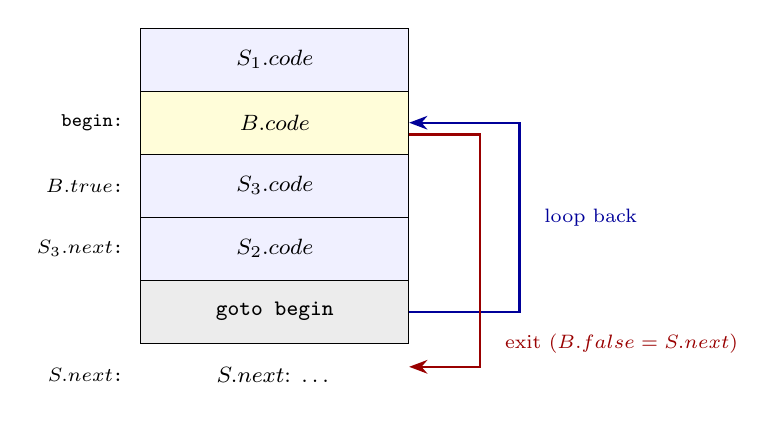
\begin{tikzpicture}[>=Stealth,font=\footnotesize,
 cell/.style={draw,minimum width=3.4cm,minimum height=0.8cm,align=center},
 lab/.style={font=\scriptsize\ttfamily,anchor=east}]
\node[cell,fill=blue!6] (s1) at (0,0) {$S_1.code$};
\node[cell,fill=yellow!15] (b) at (0,-0.8) {$B.code$};
\node[cell,fill=blue!6] (s3) at (0,-1.6) {$S_3.code$};
\node[cell,fill=blue!6] (s2) at (0,-2.4) {$S_2.code$};
\node[cell,fill=gray!15] (g) at (0,-3.2) {\texttt{goto begin}};
\node[cell,draw=none] (nx) at (0,-4.0) {$S.next$: \ldots};
\node[lab] at (-1.8,-0.8) {begin:};
\node[lab] at (-1.8,-1.6) {$B.true$:};
\node[lab] at (-1.8,-2.4) {$S_3.next$:};
\node[lab] at (-1.8,-4.0) {$S.next$:};
\draw[->,thick,blue!60!black] (g.east) -- ++(1.4,0) |- (b.east);
\draw[->,thick,red!60!black] (b.east) ++(0,-0.15) -- ++(0.9,0) |- ($(nx.east)+(0,0.1)$);
\node[font=\scriptsize,blue!60!black,anchor=west] at (3.3,-2.0) {loop back};
\node[font=\scriptsize,red!60!black,anchor=west] at (2.8,-3.6) {exit ($B.false = S.next$)};
\end{tikzpicture}
\end{document}
